%************************************************
\chapter{Theoretical background}
\label{ch:theory}
%************************************************

\section{Introduction}
Particle physics is a branch of physics that studies the most fundamental particles and their interaction.
We believe that all matter and radiation in the universe are made up of these fundamental particles, and their behaviour is described by the theories in particle physics.
In 20th century, our understanding about the nature of fundamental particles has had great breakthrough and  advance.
Also, many particle colliders have been built to give much insight to develop the theories and test the theories.
The currently mainstream theory of particle physics is called the Standard Model.

\section{Standard Model}
\label{sec:Standard_Model}
Standard Model(SM) is the current theory to describe the fundamental particles in particle physics.
It has already gained huge success in predicting the experimental results, including the prediction of existence of the top quark, the tau neutrino, and the Higgs boson.
It has also explained almost all experimental results with high accuracy.
It represents our best understanding of how the fundamental particles interact with each other.

Physicists discovered that there are 4 fundamental forces in the universe: electromagnetic force, weak force, strong force, and gravitational force.
However, SM can only describe 3 of them: electromagnetic, weak and strong interaction, and the gravity cannot be described by SM.
Figure \ref{fig:SM_particles} shows all fundamental particles in SM, and their mass, electric charge and spin.
All matter is made up of fermions (purple and green), which is the first 3 columns in figure \ref{fig:SM_particles}.
Fermions are divided into two groups: quarks(purple) and leptons(green).
The forces between the fermions are mediated by the force carriers, which is gauge bosons(red).
Higgs bosons(yellow) is scalar bosons, which give mass to other massive particles.

\begin{figure}
\centering
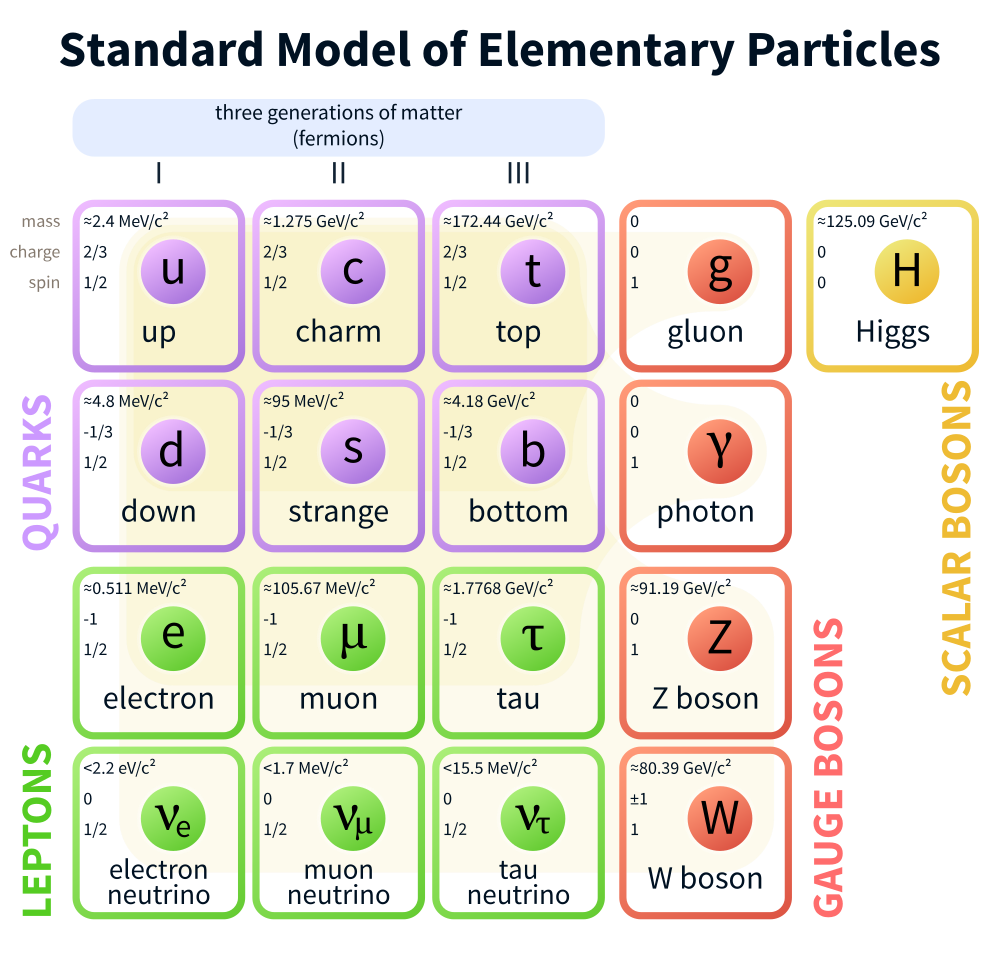
\includegraphics[width=\textwidth]{data/photo/theory/SM_particles.png}
\caption{The table for all fundamental particles in SM. \cite{SM_particles}}
\label{fig:SM_particles}
\end{figure}

\subsection{Matter particles}
There are 6 types of quarks: up quarks(u), down quarks(d), charm quarks(c), strange quarks(s), top quarks(t) and bottom quarks(b).
Quarks interact with strong interaction, while leptons does not.
There are 3 types of charged leptons: electrons, muons and taus.
There are 3 types of neutral leptons: electron neutrinos, muon neutrinos and tau neutrinos.
The first column is the first generation, which is the lightest and most stable particles.
Hence, normal matter in our daily life is made from the particles in the first generation.
The second and third column are the second and third generation respectively, which is heavier and less stable particles.
These particles will finally decay into the particles in the first generation.
Due to the phenomenon of neutrino oscillation, neutrinos should have non-zero masses, but their value are still uncertain in our current technology.

\subsection{Forces and carrier particles}
Photon is the force carrier for electromagnetic interaction.
Gluon is the force carrier for strong interaction.
Z and W bosons are the force carriers for weak interaction.
The effects of these fundamental forces stem from the exchange of the corresponding force carrier.
These forces also have different strengths and different ranges.
Strong force is the strongest force, while the electromagnetic force is in the middle.
The weak force is the weakest force among the three, but it still much much stronger than the gravity.
The electromagnetic force has infinite range, while the strong and weak forces have very short ranges at the level of subatomic particles.

For example, a proton is composed of two up quarks and one down quark, and a neutron is composed of one up quark and two down quarks.
The forces between quarks inside the proton are mediated by gluons.

\subsection{Feynman diagram}
The fundamental interactions among these fundamental particles are described by the allowed fundamental Feynman vertices.
All allowed fundamental Feynman vertices in SM are shown in figures \ref{fig:vertices_SM} and \ref{fig:vertices_higgs}.
These fundamental vertices are the basic building blocks for all physical processes, by jointing these vertices together.

\begin{figure}
\centering
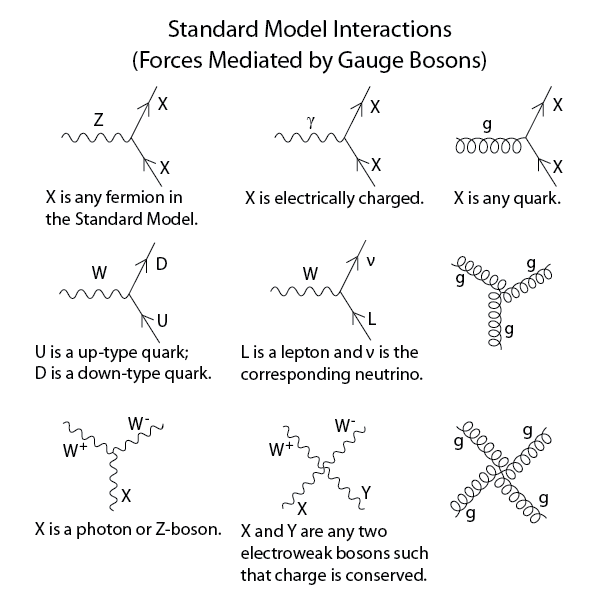
\includegraphics[width=\textwidth]{data/photo/theory/vertices_SM.png}
\caption{All allowed fundamental Feynman vertices in SM, except higgs-related vertices. \cite{vertices_SM}}
\label{fig:vertices_SM}
\end{figure}

\begin{figure}
\centering
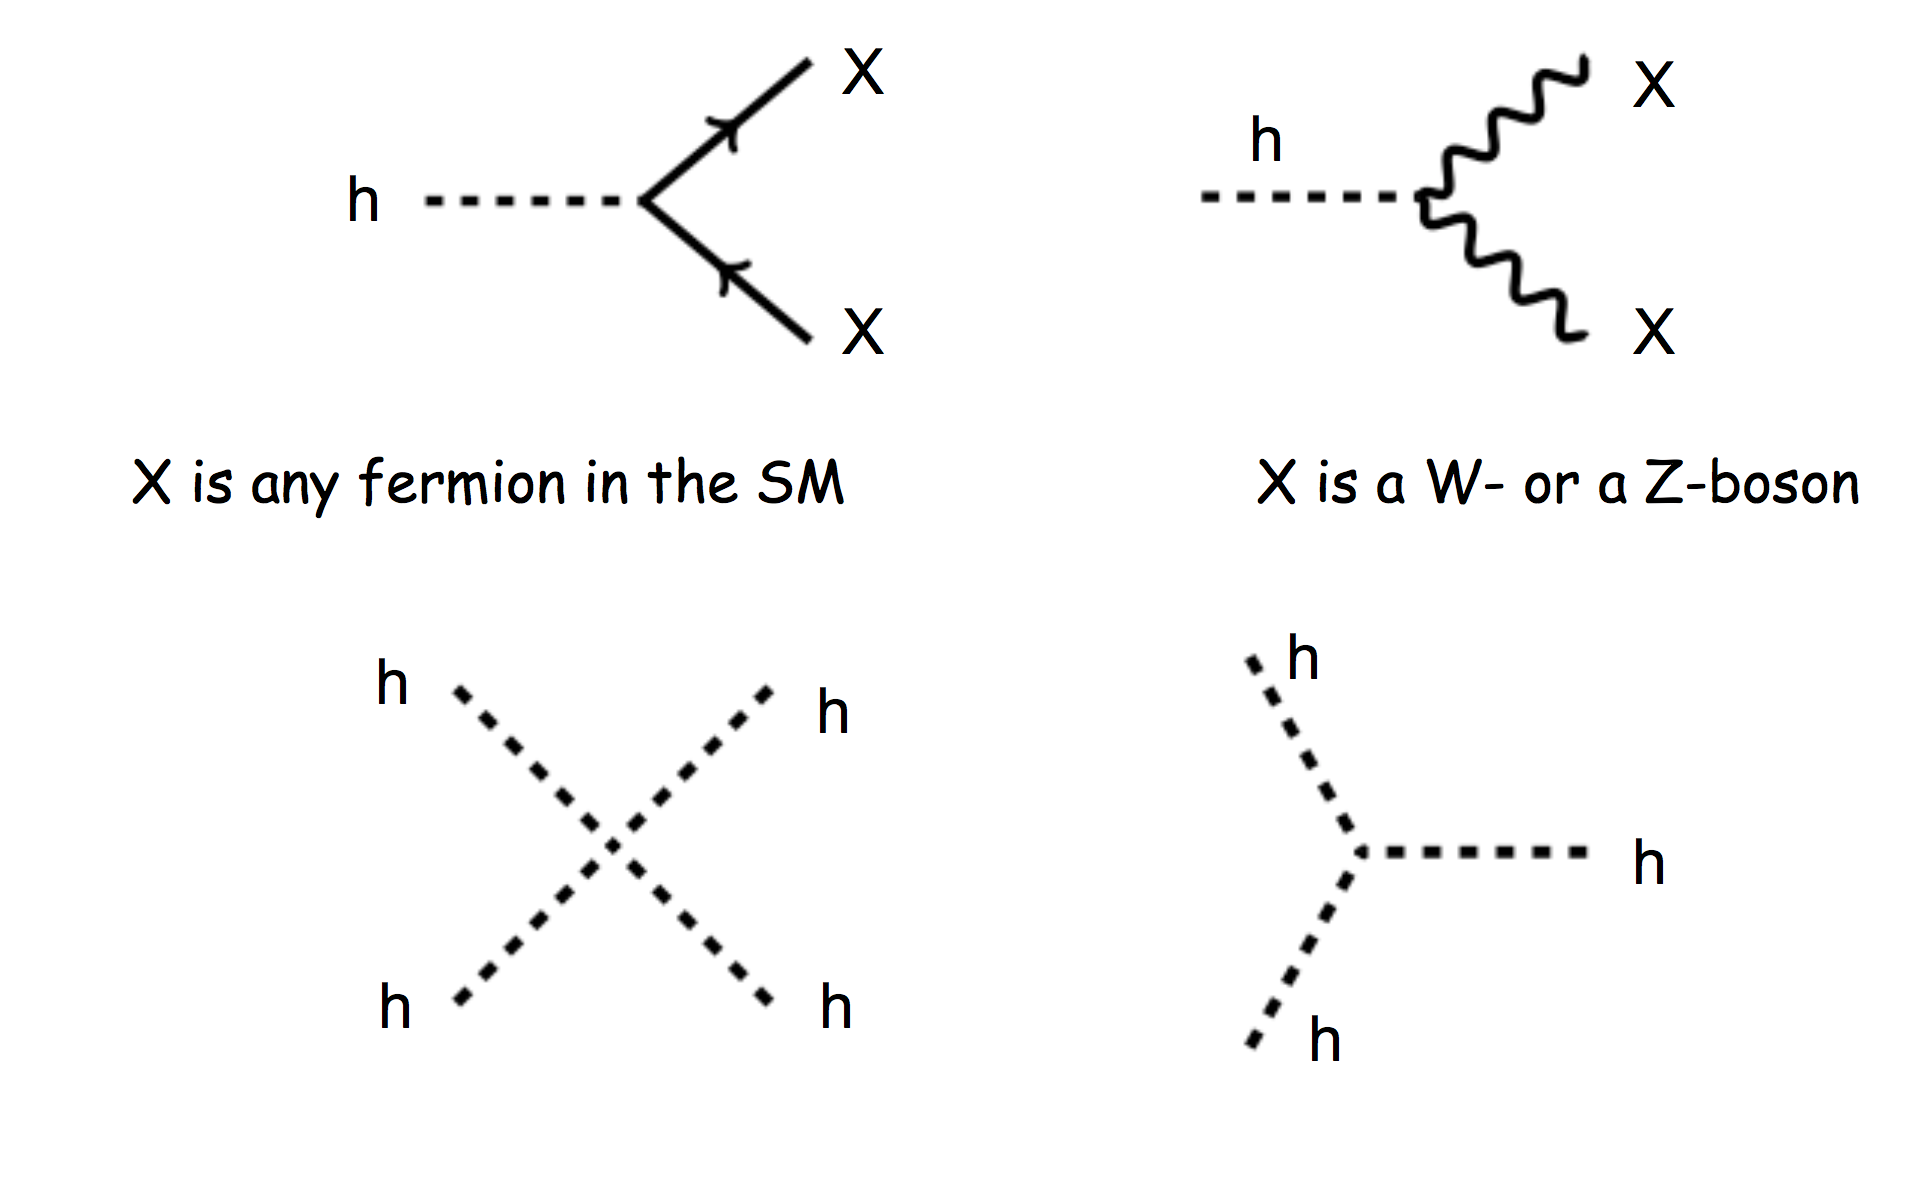
\includegraphics[width=\textwidth]{data/photo/theory/vertices_higgs.png}
\caption{All allowed fundamental higgs-related Feynman vertices in SM.}
\label{fig:vertices_higgs}
\end{figure}

\section{Limitation of Standard Model}
\label{sec:Limitation_Standard_Model}
Although Standard Model can explain almost all experimental results, there still are some phenomena it cannot explain.

\subsection{Dark matter}
\label{sec:dark_matter}
Dark matter is some unknown matter that does not involve in electromagnetic interaction, but involve in gravitational interaction.
It was first discovered in the Milky Way, by studying the speed of the stars orbiting around the center of the Milky Way.
Because it does not involve in electromagnetic interaction, it does not emit any electromagnetic radiation, and it cannot be seen by our telescopes.
However, SM cannot explain the nature of dark matter, and what dark matter is made of.

\subsection{Hierarchy problem}
\label{subsec:hierarchy_problem}
The hierarchy problem is the question why the weak force is stronger than the gravitational force by $10^{24}$ times.
It is also asked why the mass of Higgs boson ($\sim 125$ GeV) is much lighter than the Planck mass ($\sim 10^{19}$ GeV).

The Lagrangian for the interaction term between the fermion Dirac field $\psi$ and the Higgs field $h$ (i.e. Yukawa interaction) is given by
\begin{equation}
\mathcal{L}_{\text{Yukawa}} = - \lambda \bar{\psi} h \psi
\end{equation}
where $\lambda$ is the Yukawa coupling constant.
The quantum correction to the square of the Higgs mass $\Delta m^2_H$ is then given by
\begin{equation}
\Delta m^2_H = - \frac{|\lambda|^2}{16 \pi^2} \Lambda^2 + \dots
\label{eq:higgs_correction}
\end{equation}
where $\Lambda$ is the energy scale up to which the Standard Model is valid, namely the Planck scale ($\sim 10^{19}$ GeV).
Because $\Lambda$ is quadratic divergent, the correction to the Higgs mass is in the order of Planck scale.
Unless there are very delicate cancellation between the correction terms, the Higgs mass should be in the order of Planck scale.
But, we found that the experimental Higgs mass is in the order of 125 GeV, and this is called the hierarchy problem.

\subsection{Unification of forces}
In the 1860s, James Clerk Maxwell wrote down his famous equations Maxwell's equations, which unified two different phenomena: electricity and magnetism.
Due to this unification, we now understand that electricity and magnetism are two different manifestations of the same phenomenon, and we now call it electromagnetism.

Similar thing happened in the 1970s, physicists developed a theory that unified two fundamental forces: electromagnetic force and weak force.
At the energy scale above 246 GeV, these two forces will merge into a single force: electroweak force.
This unification predicted the existence of weak neutral current and a force carrier to carry this weak force.
This force carrier was later confirmed experimentally in CERN, and it is now called the Z boson.

After that, an effect of strong force was found experimentally that the strong force becomes weaker when the energy is higher.
This may indicate that electroweak force and strong force will become a single force at even high energy.
However, the energy scale at which these forces are the same is much larger than the energy the particle accelerators can reach.
There are some theories beyond the Standard Model that try to unify these forces, such as supersymmetry.

\section{Supersymmetry}
Supersymmetry(SUSY) is an extension of the Standard Model, and try to answer some questions which the Standard Model cannot explain, mentioned in section \ref{sec:Limitation_Standard_Model}.
One of the problems SUSY can solve is the hierarchy problem of Higgs mass mentioned in section \ref{subsec:hierarchy_problem}.
We first notice that the negative sign in the equation \ref{eq:higgs_correction} is due to the correction from the fermions.
If we can somehow have a symmetry between the fermions and bosons, and add more positive correction terms due to the bosons, the correction terms will cancel with each other and the hierarchy problem can be solved.
This new symmetry is called the supersymmetry (SUSY).

\subsection{Minimal Supersymmetric Standard Model}
Minimal Supersymmetric Standard Model(MSSM) is the simplest realization of the supersymmetric theories that contain the minimum number of new particles and new interactions.
It predicts that each particle in the Standard Model has its own partner particle, called the superpartner, as shown in figure \ref{fig:SUSY_particles}.
The name of the superpartner of a fermion is by adding a prefix ``s'', followed by the name of the original Standard Model particle: squarks and sleptons, etc.
For example, the superpartner of an electron is called selectron.
For the superpartner of a Standard Model boson, the suffix ``ino'' is added: gluino and Higgsino, etc.
As for the symbol for the superpartner, a tilde will be added above the original symbol.
For example, the symbol for selectron is $\tilde{e}$.
Also, the spin of the superpartner will differ from the Standard Model particle by 1/2.
For fermions, the spin of their superpartner is 0, while for bosons, the spin of their superpartner is 1/2.
The superpartners would interact with the same forces as the Standard Model particles, but they would have different masses.
This is the new symmetry between the fermions and bosons, mentioned before.
It is also the correction terms from these superpartners to fix the hierarchy problem of the Higgs mass.

\begin{figure}
\centering
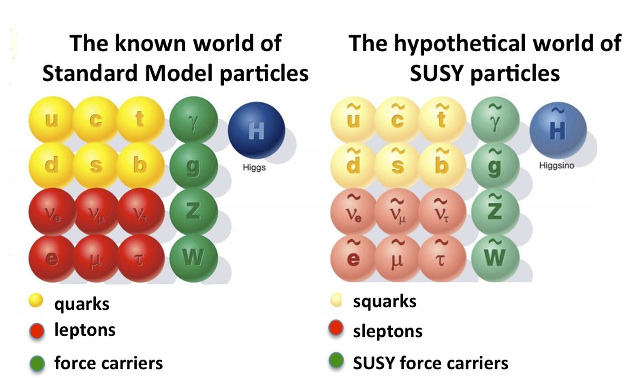
\includegraphics[width=\textwidth]{data/photo/theory/SM-SUSY-diagram.jpg}
\caption{The particles in Standard Model and their corresponding superpartners and their names}
\label{fig:SUSY_particles}
\end{figure}

In the MSSM, one neutral Higgs boson $H$ and two charged Higgs bosons $H^+$, $H^-$ needed to be introduced.
This means that for the Standard Model electro-weak bosons, there are 4 neutral bosons: $\gamma$, $Z$, $h$ and $H$, and 4 charged bosons: $W^+$, $W^-$, $H^+$ and $H^-$.
The superpartners of the 4 neutral bosons together form 4 mass eigenstates, called neutralinos: $\tilde{\chi}_1^0$, $\tilde{\chi}_2^0$, $\tilde{\chi}_3^0$ and $\tilde{\chi}_4^0$.
The superpartners of the 4 charged bosons together form two mass eigenstates with electric charge $\pm 1$, called charginos: $\tilde{\chi}_1^\pm$ and $\tilde{\chi}_2^\pm$.
The subscripts of the symbol of the neutralinos and charginos are labeled by the ascending order in mass.
Table \ref{tab:SUSY_particle} summarizes the Standard Model particles and their superpartners.
If MSSM is correct, these supersymmetric particles should be detected in the LHC.

\begin{table}[htbp]
\tiny
\centering
\begin{tabular}{|c|cccc|cccc|}
\hline
\hline
Type & SM particle & Symbol & Spin & R-parity & Superpartner & Symbol & Spin & R-parity \\
\hline
\hline
Fermions & Quark  & $q$ & $\frac{1}{2}$ & +1 & Squark  & $\tilde{q}$ & 0 & -1 \\
         & Lepton & $l$ & $\frac{1}{2}$ & +1 & Slepton & $\tilde{l}$ & 0 & -1 \\
\hline
Gluon & Gluon  & $g$ & $1$ & +1 & Gluino & $\tilde{g}$ & $\frac{1}{2}$ & -1  \\
\hline
Neutral EW Bosons & Photon         & $\gamma$ & $1$ & +1
                  &  &  &  &  \\
                  & Z Boson        & $Z$      & $1$ & +1
                  & Neutralinos & $\tilde{\chi}_1^0$, $\tilde{\chi}_2^0$, $\tilde{\chi}_3^0$, $\tilde{\chi}_4^0$ & $\frac{1}{2}$ & -1 \\
                  & Neutral Higgs  & $h$,$H$  & $0$ & +1
                  &  &  &  &  \\
\hline
Charged EW Bosons & W Boson        & $W^+$, $W^-$  & $1$ & +1
                  & Charginos & $\tilde{\chi}_1^\pm$, $\tilde{\chi}_2^\pm$ & $\frac{1}{2}$ & -1 \\
                  & Charged Higgs  & $H^+$, $H^-$  & $0$ & +1
                  &  &  &  &  \\
\hline
\hline
\end{tabular}
\caption{The spin and R-parity for the Standard Model particles and their superpartners.}
\label{tab:SUSY_particle}
\end{table}

The baryon number $B$ is defined by $\frac{1}{3} (n_q - n_{\bar{q}})$, where $n_q$ is the number of quarks and $n_{\bar{q}}$ is the number of anti-quarks.
The lepton number $L$ is defined by $n_l - n_{\bar{l}}$, where $n_l$ is the number of leptons and $n_{\bar{l}}$ is the number of anti-leptons.
In the Standard Model and the experimental data, $B-L$ is conserved, but in MSSM, it is no longer conserved.
To keep this conservation and prevent the proton decay, the R-parity $P_R$ is introduced.
\begin{equation}
P_R = (-1)^{3(B-L)-2s}
\end{equation}
where s is the spin.
By this definition, all Standard Model particles have R-parity $+1$, and all supersymmetric particles have R-parity $-1$.
If the R-parity is conserved, the lightest supersymmetric particle (LSP) cannot decay and is stable.
If the LSP is electrically neutral and interacts with matter only by the weak interaction and gravity, for example the lightest neutralinos $\tilde{\chi}_1^0$ or a sneutrino $\tilde{\nu}$, it could be a candidate for dark matter mentioned in section \ref{sec:dark_matter}.
In this thesis, the R-parity is assumed to be conserved, and the lightest neutralino $\tilde{\chi}_1^0$ is assumed to be the LSP.
Due to the conservation of R-parity, the supersymmetric particles can only be pair-produced, and will eventually decay into Standard Model particles and the lightest neutralino $\tilde{\chi}_1^0$, i.e. the LSP in this thesis.

\section{Signal scenario}
\label{sec:Wh_signal}
In the recent searches for the squarks and gluinos, the masses of gluinos and the first and second generation squarks are suggested to be larger than 1 TeV, while the masses of the third generation squarks are still allowed to be below 1 TeV \cite{gluinos}.
In this case, the direct pair production of electroweak gauginos (i.e. neutralinos and charginos) may be the dominant SUSY production process at the LHC, if the masses of the gluinos and squarks are significantly heavier than the low mass electroweak gauginos, because the production cross sections of supersymmetric particles depend on the masses of the sparticles.
With the results in the Run-I analysis \cite{run1} by using the center-of-mass energy $\sqrt{s} = 8$ TeV shown in figure \ref{fig:result_run1}, the electroweak pair production may be a promising hope for SUSY discovery at a higher center-of-mass energy $\sqrt{s} = 13$ TeV in Run-II using 2015 and 2016 data.

\begin{figure}
\centering
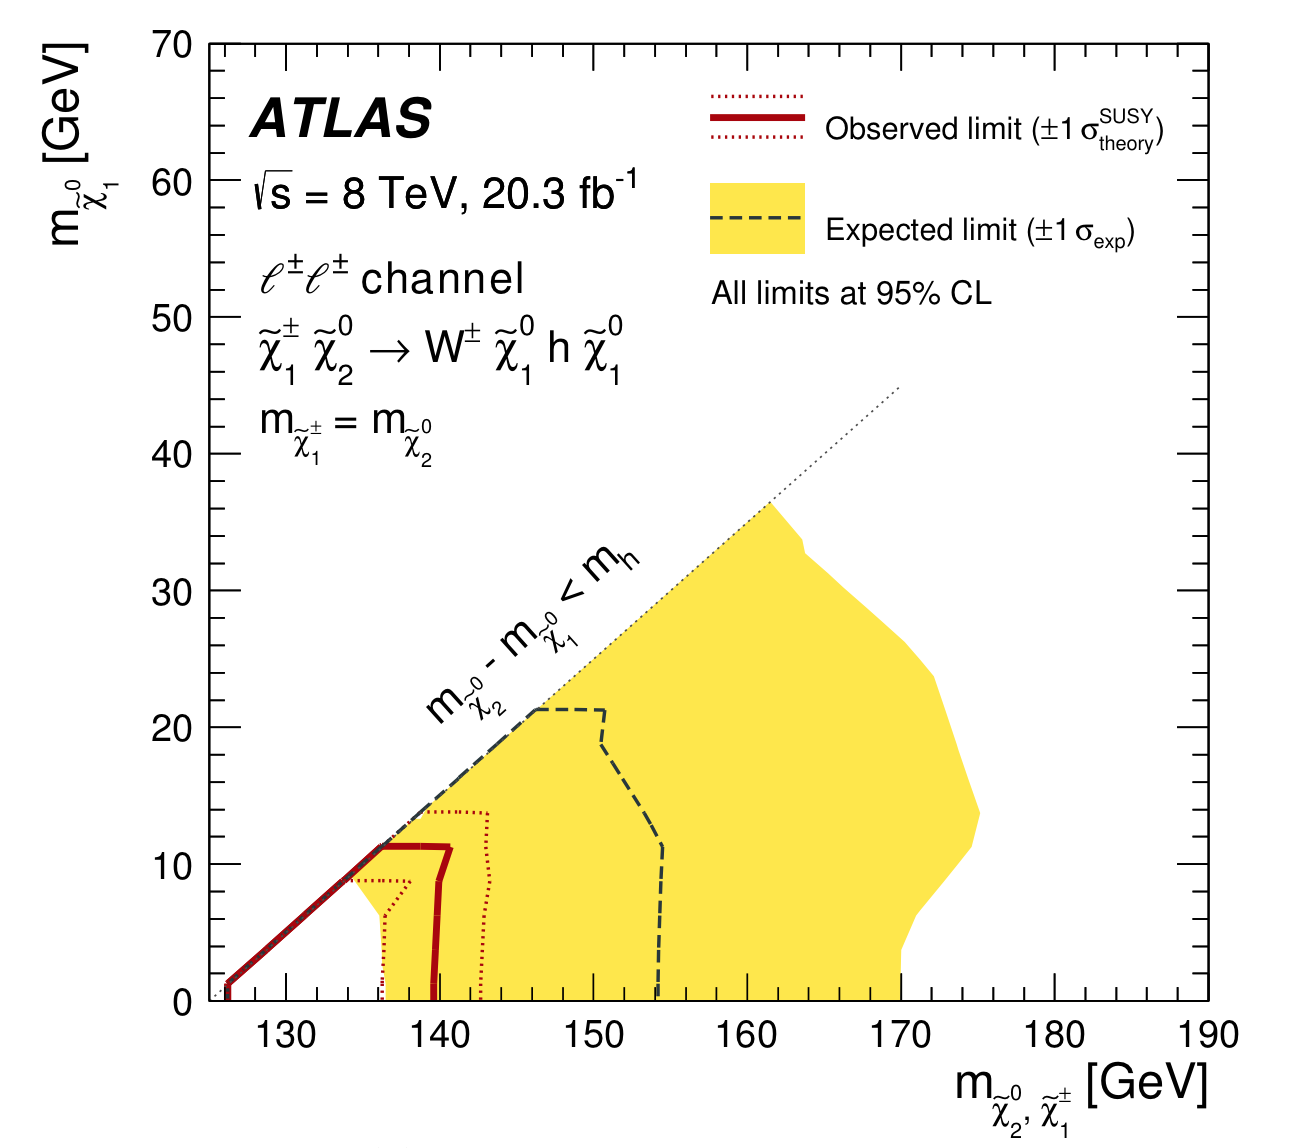
\includegraphics[width=0.5\textwidth]{data/photo/theory/run1.png}
\caption{The exclusion contours for the masses $m_{\tilde{\chi}_1^\pm , \tilde{\chi}_2^0}$ and $m_{\tilde{\chi}_1^0}$ in the Run-I analysis \cite{run1}.}
\label{fig:result_run1}
\end{figure}

Same as the Run-I analysis, the supersymmetric process we are looking for is the pair production of the lightest chargino $\tilde{\chi}_1^\pm$ and the second lightest neutralino $\tilde{\chi}_2^0$.
The masses of them are assumed to be the same, $m_{\tilde{\chi}_1^\pm} = m_{\tilde{\chi}_2^0}$, and denoted by $m_{\tilde{\chi}_1^\pm , \tilde{\chi}_2^0}$ in the later chapters.
With the assumption that all sleptons are heavier than $\tilde{\chi}_1^\pm$ and $\tilde{\chi}_2^0$,
$\tilde{\chi}_1^\pm$ will decay to W boson and $\tilde{\chi}_1^0$ (i.e. $\tilde{\chi}_1^\pm \rightarrow W^{\pm} + \tilde{\chi}_1^0$)
and $\tilde{\chi}_2^0$ will decay to the lightest MSSM Higgs boson $h$ and $\tilde{\chi}_1^0$ (i.e. $\tilde{\chi}_2^0 \rightarrow h + \tilde{\chi}_1^0$),
or Z boson and $\tilde{\chi}_1^0$ (i.e. $\tilde{\chi}_2^0 \rightarrow Z + \tilde{\chi}_1^0$).
In this thesis, we assume $\tilde{\chi}_1^\pm \rightarrow W^{\pm} + \tilde{\chi}_1^0$ and $\tilde{\chi}_2^0 \rightarrow h + \tilde{\chi}_1^0$ decays with 100\% branching ratio, which is the Wh channel we are looking for.
The mass of the lightest MSSM Higgs boson $h$ is set to 125 GeV.

The W boson from $\tilde{\chi}_1^\pm$ will decay into one lepton (electron or muon) and one neutrino (i.e. $W{^\pm} \rightarrow \ell^{\pm} + \nu$) with the SM branching ratio.
The Higgs boson form $\tilde{\chi}_2^0$ will eventually decay into one lepton (electron or muon), quarks (i.e. jets) and neutrino(s) by various decay modes with the SM branching ratios.
For example, $h \rightarrow W^{+} W^{-} $ and $h \rightarrow \tau^{+} \tau^{-} $ are the dominant decay modes, with one of the $W / \tau$ decays leptonically (e.g. $W{^\pm} \rightarrow \ell^{\pm} + \nu$) and another decays hadronically (e.g. $W \rightarrow q + q$).
The Feynman diagram in figure \ref{fig:signal_feynman} summarizes the whole signal scenario we are looking for in this thesis.

\begin{figure}
\centering
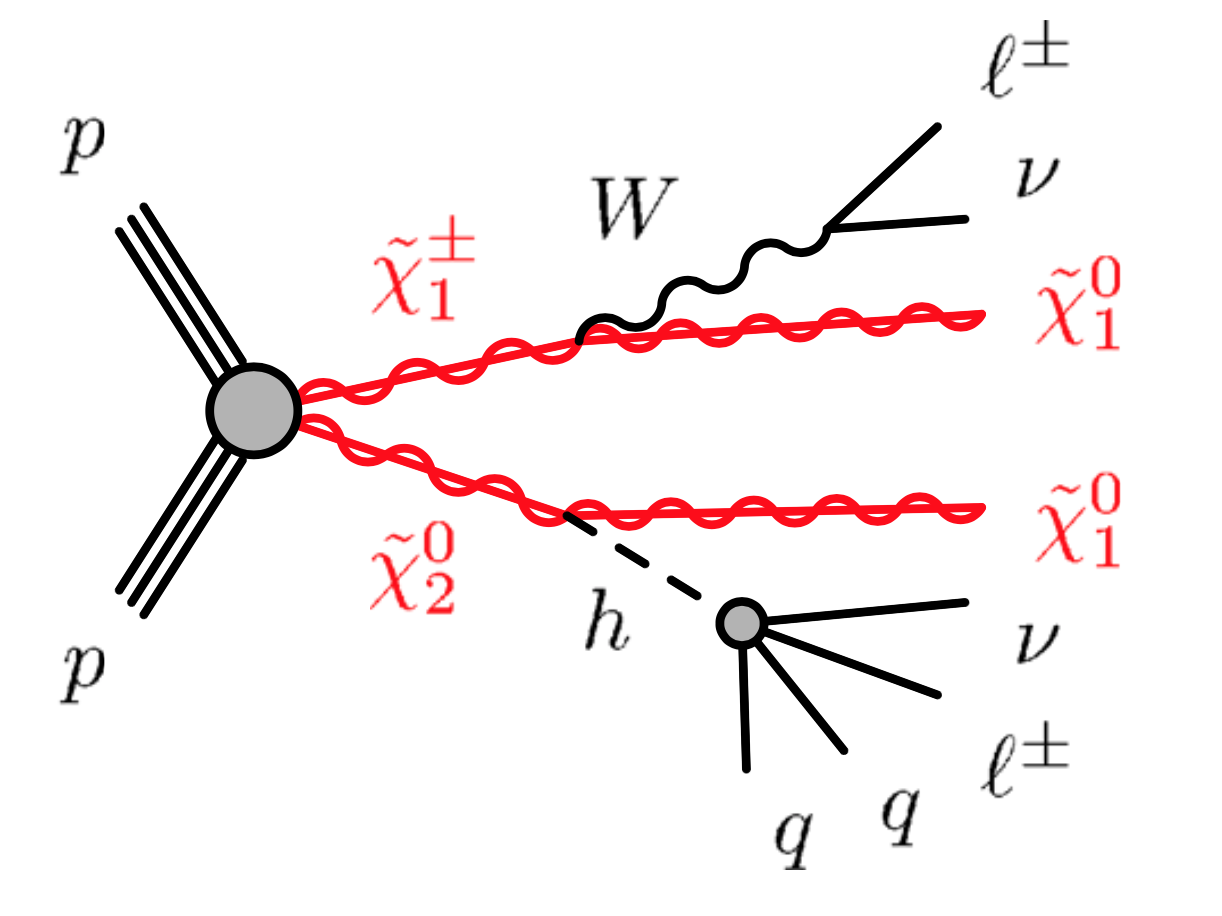
\includegraphics[width=0.5\textwidth]{data/photo/theory/signal_feynman.png}
\caption{The Feynman diagram for the Wh same-sign signal scenario in this thesis. The final states in this process are two same-sign leptons (electron or muon), quarks (i.e. jets) and missing transverse momentum contributed by the lightest neutralinos $\tilde{\chi}_1^0$ and neutrinos $\nu$.}
\label{fig:signal_feynman}
\end{figure}

The two leptons in the final states are either electrons or muons, and the term ``lepton'' (with symbol $\ell$) in the later chapters in this thesis refers to electron or muon, but not tau lepton or neutrino.
We are only looking for two leptons with the same electric charge, in order to suppress the Standard Model backgrounds that have two leptons with opposite electric charge, mainly from Z boson decays.
The mass splitting between the two lightest neutralinos ($m_{\tilde{\chi}_2^0} - m_{\tilde{\chi}_1^0}$) should be larger that the mass of Higgs boson ($\sim$ 125 GeV), in order to be able to pass the requirement of the signal lepton ($p_T > 25$ GeV), described in table \ref{tab:lepdef}.
In the case that mass splitting is close to the mass of Higgs boson, which is called the compressed region, one of the lepton may not pass the requirement of the signal lepton, due to the low momentum of the Higgs boson.
However, if the Higgs boson eventually decays into two leptons, for example $h \rightarrow ZZ$ with one of the Z boson decays leptonically (e.g. $Z \rightarrow \ell^{+} + \ell^{-}$) and another decays hadronically (e.g. $Z \rightarrow q + q$), the total number of leptons in the final state will be three.
If one of the three leptons has low momentum and does not pass the signal requirement (i.e. not detected), and another two leptons have the same electric charge, this scenario will have the same final state as our signal.
This means that in the compressed region, there are more decay modes for the Higgs boson, such that they have the same final state in our signal scenario, and hence this will contribute more sensitivity in the compressed region.

Because the two neutralinos $\tilde{\chi}_1^0$ and neutrinos $\nu$ in the final state cannot be detected, a large missing transverse momentum (i.e. unbalanced momentum in the detector) will be expected.
This is also a signature for our signal.

This analysis is a collaborative work with other people and the results are mainly based on the paper \cite{Wh} and the internal note \cite{WhSS}.
